\documentclass[11pt]{article}
\usepackage[margin = 1in]{geometry}
\usepackage{amsmath}
\usepackage{amssymb}
\usepackage{amsthm}
\usepackage{graphicx}
\usepackage{subfig}
\usepackage{enumitem}
\usepackage{url}
\usepackage[parfill]{parskip}
\newcommand{\skipline}{\vspace{\baselineskip}}
\newcommand{\bmath}[1]{\boldmath#1\unboldmath}
\newcommand{\bmathIT}[1]{\text{\boldmath#1\unboldmath}}
\newenvironment{problem}[1]{\textbf{Problem #1: }}{\newpage}


\begin{document}

	\begin{center}
		\textbf{Midterm 1} \\
		\textbf{Ordinary Differential Equations} \\
		\textbf{Math 537} \\
		\textbf{Stephen Giang RedID: 823184070} \\
		\skipline \skipline
	\end{center}

	\begin{problem}{1}
		The well-known ”SIR” epidemic model (Kermack and McKendrick, 1927) consists of three first-order ordinary differential equations (ODEs) for three time dependent variables, $S, I$, and $R$, that represent susceptible, infected, and recovered individuals, respectively. In HW2, we have reduced the system of three ODEs into a single ODE with one time
		dependent variable $R$, as follows:
		\[\frac{dR}{dt} = \nu \left(N - R - S(0)e^{-\frac{\beta}{N \nu}(R(t) - R(0))}\right). \tag{1.1}\]
		Here, three parameters, $\beta > 0$, $\nu > 0$, and $N > 0$, represent a transmission rate, a recovery rate, and a fixed population $(N = S + I + R)$, respectively. $S(0)$ and $R(0)$ denote the initial values of $S$ and $R$, respectively. Complete the following problems.
		\\ \\
		\begin{enumerate}[label = (\alph*)]
			\item Consider the following logistic equation:
			\[\frac{df}{dt} = f(1-f) \tag{1.2}.\]
			Introduce a new dependent variable $(g)$ to transform Eq. (1.2) into the following ODE:
			\[\frac{dg}{dt} = \frac{1}{4} - g^2. \tag{1.3}\]
			\\ \\
			Notice the following:
			\begin{align*}
				\frac{dg}{dt} &= \frac{1}{4} - g^2 \\
				&= \left(\frac{1}{2} + g\right)\left(\frac{1}{2} - g\right) \\
				&= \left(\frac{1}{2} + g\right)\left(1 - \left(\frac{1}{2} + g\right)\right) \\
				&= f (1 - f) \\
				&= \frac{df}{dt}
			\end{align*}
			Notice that if we let $f = \frac{1}{2} + g$, or let $g = f - \frac{1}{2}$, we get that $\frac{dg}{dt} = \frac{df}{dt}$, so we can transform Eq (1.2) to Eq (1.3)
			\newpage
			
			\item Express the solutions of Eqs. (1.2) and (1.3) in terms of the sigmoid and hyperbolic tangent functions, respectively.
			\\ \\
			Notice we can solve equation (1.2)  through the use of Bernoulli's.  Let $u = \frac{1}{f}$, with $\frac{du}{dt} = \frac{-1}{f^2} \frac{df}{dt}$
			\begin{align*}
				\frac{df}{dt} - f &= -f^2 & \int \frac{du}{1 - u} &= \int dt \\
				\frac{-1}{f^2} \frac{df}{dt} + \frac{1}{f} &= 1 & -\ln(1-u) &= t + C \\
				\frac{du}{dt} + u &= 1 & u &= 1 + Ce^{-t} \\
			\end{align*}
			After resubstitution we get that \bmath{\[f = \frac{1}{1 + Ce^{-t}}\]} Notice that this is in terms of the Sigmoid function: $S(x) = \frac{1}{1 + e^{-x}}$
			\\ \\ \\ \\
			Notice we can solve equation (1.3) by Separation:
			\begin{align*}
				\frac{dg}{dt} &= \frac{1}{4} - g^2 & 2 \tanh^{-1} (2g) &= t + C \\
				\frac{4\,dg}{1 - 4g^2} &= dt & 2g &= \tanh \frac{t + C}{2} \\
				2 \int \frac{2 \, dg}{1 - (2g)^2} &= \int dt 
			\end{align*}
			Thus we get that
			\bmath{\[g = \frac{1}{2}\tanh \frac{t + C}{2}\]}
			Notice that this is in terms of the hyperbolic tangent function.
			\newpage
			\item  Apply a Taylor series expansion with $e^{-x} \approx 1 - x + \frac{x^2}{2}$ to simplify the term $e^{-\frac{\beta}{N \nu}(R(t) - R(0))}$ in Eq. (1.1). Then, perform a (linear) stability analysis.
			\\ \\
			Notice we can convert the exponential part of equation (1.1) to its 2nd-order Taylor polynomial counterpart.  So we get that:
			\[e^{-\frac{\beta}{N \nu}(R(t) - R(0))} \approx 1 - \frac{\beta}{N \nu}(R(t) - R(0)) + \frac{\left(-\frac{\beta}{N \nu}(R(t) - R(0))\right)^2}{2}\]
			So we can now have the following for equation (1.1):
			\begin{align*}
			\frac{dR}{dt} &\approx  \nu \left(N - R - S(0) \left( 1 - \frac{\beta}{N \nu}(R(t) - R(0)) + \frac{1}{2}\left(\frac{\beta}{N \nu}(R(t) - R(0))\right)^2\right) \right) \\
			&\approx \left(N\nu - R\nu - S(0)\nu \left( 1 - \frac{\beta}{N \nu}(R(t) - R(0)) + \frac{1}{2}\left(\frac{\beta}{N \nu}(R(t) - R(0))\right)^2\right) \right) \\
			&\approx \left(N\nu - R\nu - S(0)\nu \left( 1 - \frac{\beta}{N \nu}(R(t) - R(0)) + \frac{\beta^2}{2 N^2 \nu^2}(R(t) - R(0))^2 \right) \right) \\
			&\approx N\nu - R\nu - S(0)\nu + \frac{\beta S(0)}{N}(R(t) - R(0)) - \frac{\beta^2 S(0)}{2 N^2 \nu}(R(t) - R(0))^2 \\
			&\approx N\nu - \nu(R(t) - R(0)) - R(0)\nu - S(0)\nu + \frac{\beta S(0)}{N}(R(t) - R(0)) - \frac{\beta^2 S(0)}{2 N^2 \nu}(R(t) - R(0))^2 \\
			&\approx \left(N\nu - R(0)\nu - S(0)\nu\right) + \bmathIT{$\left(\frac{\beta S(0)}{N}-\nu\right)(R(t) - R(0))$} - \frac{\beta^2 S(0)}{2 N^2 \nu}(R(t) - R(0))^2 
			\end{align*}
			Notice that this is in form of:
			\[\frac{dx}{dt} = f(x_c) + f'(x_c)(x-x_c) + \cdots \]
			This means that at a critical point we have:
			\[\frac{dR}{dt} = \left(\frac{\beta S(0)}{N}-\nu\right)(R(t) - R(0)) + \cdots \]
			So we get that the critical point is unstable if $\left(\frac{\beta S(0)}{N}-\nu\right) > 0$, and stable if $\left(\frac{\beta S(0)}{N}-\nu\right) < 0$
			\newpage
			\item  Solve the ODE derived in problem (1c) using a small nonnegative, $R(0)$.
			\\ \\
			For small nonnegative values of $R(0)$, we can say that:
			\[\frac{dR}{dt} = \left(\frac{\beta S(0)}{N}-\nu\right)(R(t) - R(0))\]
			This is solvable by separation:
			\begin{align*}
				\int \frac{dR}{R(t) - R(0)} &= \int \left(\frac{\beta S(0)}{N}-\nu\right) dt \\
				\ln (R(t) - R(0) ) &= \left(\frac{\beta S(0)}{N}-\nu\right) t + C \\
				R(t) - R(0) &= Ce^{\left(\frac{\beta S(0)}{N}-\nu\right) t} \\
				R(t) &= Ce^{\left(\frac{\beta S(0)}{N}-\nu\right) t} + R(0)
			\end{align*}
		\end{enumerate}
	\end{problem}

	\begin{problem}{2}
		A nonlinear, non-dissipative Lorenz model is written as follows:
		\[\frac{d^2X}{dt^2} - (\sigma r  + C)X + \frac{X^3}{2} = 0\,.\tag{2}\]
		Here, we assume that both $\sigma$ and $r$ are positive, and choose $C = 0$ for convenience. Complete the following problems.
		\begin{enumerate}[label = (\alph*)]
			\item Transform the 2nd order ODE in Eq. (2) into a system of first order ODEs, (i.e., $Y = X'$).
			\\ \\
			First, we can substitute the values given, and isolate the second derivative to get the following:
			\[\frac{d^2X}{dt^2} = \sigma rX - \frac{X^3}{2}\]
			Now notice if we let $Y = X'$ and $Y' = X''$, we get the following system:
			\[
			\bmathIT{$y$} = 
			\begin{pmatrix}
				Y \\ Y'
			\end{pmatrix} =
			\begin{pmatrix}
				0 & 1 \\
				\sigma r - \frac{X^2}{2} & 0
			\end{pmatrix}
			\begin{pmatrix}
				X \\ X'
			\end{pmatrix} =  \bmathIT{$Ax$}
			\]
			Where \bmath{$A$} $= \begin{pmatrix}
			0 & 1 \\
			\sigma r - \frac{X^2}{2} & 0
			\end{pmatrix}$, \bmath{$x$} $= \begin{pmatrix}
			X \\ X'
			\end{pmatrix}$, \bmath{$y$} $=\begin{pmatrix}
			Y \\ Y'
			\end{pmatrix}$
			\\ \\ \\
			\item Find critical points in the above 2D system in problem (2a).
			\\ \\
			We can solve for the critical points by letting \bmath{y} equal to \bmath{$\vec{0}$}.
			\[
			\begin{pmatrix}
				0 \\ 0
			\end{pmatrix} = 
			\begin{pmatrix}
			0 & 1 \\
			\sigma r - \frac{X^2}{2} & 0
			\end{pmatrix}
			\begin{pmatrix}
			X \\ X'
			\end{pmatrix}
			\]  
			So now we must find $X$ and $X'$ such that when multiplied by the rows of \bmath{$A$}, we get \bmath{$\vec{0}$}.
			To find our critical points, we need to solve the following:
			\begin{align*}
				\sigma r - \frac{X^2}{2} &= 0 & X^2 &= 2\sigma r  \\
				 \frac{X^2}{2} &= \sigma r & X &= \pm \sqrt{2\sigma r}  			
			\end{align*} 
			We set $X' = 0$, so that the critical solution multiplied with the first row of \bmath{$A$} also equals 0.
			So we get the critical points to be \bmath{$\begin{pmatrix} \sqrt{2\sigma r} \\ 0 \end{pmatrix} $}, \bmath{$\begin{pmatrix} -\sqrt{2\sigma r} \\ 0 \end{pmatrix} $}, and the trivial solution \bmath{$\begin{pmatrix} 0 \\ 0	\end{pmatrix}$}. 
			
			\newpage
			
			\item  Compute the Jacobian matrix of the above 2D system.
			\\ \\
			Notice the Jacobian:
			\[
			J(X,X') = 
			\begin{bmatrix}
				\frac{\partial Y}{\partial X} & \frac{\partial Y}{\partial X'} \\ \\
				\frac{\partial Y'}{\partial X} & \frac{\partial Y'}{\partial X'}
			\end{bmatrix} =
			\begin{bmatrix}
				0 & 1 \\
				\sigma r - \frac{3X^2}{2} & 0
			\end{bmatrix}
			\]
			\item Perform a linear stability analysis for all of the critical points.
			\\ \\
			Notice the Jacobian at the critical points:
			\[J(0,0) = \begin{bmatrix}
			0 & 1 \\ \sigma r & 0 
			\end{bmatrix}\]
			Notice we can find the characteristic equation by find the determinant of the evaluated Jacobian minus $\lambda I$.
			\begin{align*}
				\lambda^2 - \sigma r&= 0 \\
				\lambda^2 &= \sigma r \\
				\lambda &= \pm \sqrt{\sigma r}
			\end{align*}
			So we get the following eigenvalues, $\lambda_1 = \sqrt{\sigma r}, \lambda_2 = -\sqrt{\sigma r}$
			\\ \\
			Notice we can find the eigenvectors by subtracting $\lambda I$ from our evaluated Jacobian.
			\begin{align*}
				\begin{bmatrix}
				0-\lambda_1 & 1 \\ \sigma r & 0-\lambda_1 
				\end{bmatrix}\begin{bmatrix}
					X \\ X'
				\end{bmatrix} = 
				\begin{bmatrix}
				-\sqrt{\sigma r} & 1 \\ \sigma r & -\sqrt{\sigma r}
				\end{bmatrix}\begin{bmatrix}
				X \\ X'
				\end{bmatrix}, && v_1 = \begin{bmatrix}
					X \\ X'
				\end{bmatrix} = \begin{bmatrix}
					1 \\ \sqrt{\sigma r}
				\end{bmatrix}
				\\
				\begin{bmatrix}
				0-\lambda_2 & 1 \\ \sigma r & 0-\lambda_2
				\end{bmatrix}\begin{bmatrix}
				X \\ X'
				\end{bmatrix} = 
				\begin{bmatrix}
				\sqrt{\sigma r} & 1 \\ \sigma r & \sqrt{\sigma r}
				\end{bmatrix}\begin{bmatrix}
				X \\ X'
				\end{bmatrix}, && v_2 = \begin{bmatrix}
				X \\ X'
				\end{bmatrix} = \begin{bmatrix}
				1 \\ -\sqrt{\sigma r}
				\end{bmatrix}
			\end{align*}
			The opposite eigenvalues dictate a \textbf{half-stable saddle point}
			\[J(\pm \sqrt{2\sigma r},0)= \begin{bmatrix}
			0 & 1 \\ -2\sigma r & 0 
			\end{bmatrix}\]
			Notice we can find the characteristic equation by find the determinant of the evaluated Jacobian minus $\lambda I$.
			\begin{align*}
				\lambda^2 + 2\sigma r &= 0 \\
				\lambda^2 &= -2\sigma r \\
				\lambda &= \pm \sqrt{-2\sigma r}
			\end{align*}
			So we get the following eigenvalues, $\lambda_1 = i\sqrt{2\sigma r}, \lambda_2 = -i\sqrt{2\sigma r}$
			\\ \\
			Notice we can find the eigenvectors by subtracting $\lambda I$ from our evaluated Jacobian.
			\begin{align*}
			\begin{bmatrix}
			0-\lambda_1 & 1 \\ -2\sigma r & 0-\lambda_1 
			\end{bmatrix}\begin{bmatrix}
			X \\ X'
			\end{bmatrix} = 
			\begin{bmatrix}
			-i\sqrt{2\sigma r} & 1 \\ -2\sigma r & -i\sqrt{2\sigma r}
			\end{bmatrix}\begin{bmatrix}
			X \\ X'
			\end{bmatrix}, && v_1 = \begin{bmatrix}
			X \\ X'
			\end{bmatrix} = \begin{bmatrix}
			1 \\ i\sqrt{2\sigma r}
			\end{bmatrix}
			\\
			\begin{bmatrix}
			0-\lambda_2 & 1 \\ -2\sigma r & 0-\lambda_2
			\end{bmatrix}\begin{bmatrix}
			X \\ X'
			\end{bmatrix} = 
			\begin{bmatrix}
			i\sqrt{2\sigma r} & 1 \\ -2\sigma r & i\sqrt{2\sigma r}
			\end{bmatrix}\begin{bmatrix}
			X \\ X'
			\end{bmatrix}, && v_2 = \begin{bmatrix}
			X \\ X'
			\end{bmatrix} = \begin{bmatrix}
			1 \\ -i\sqrt{2\sigma r}
			\end{bmatrix}
			\end{align*}
			The complex eigenvalues with no real parts dictate a \textbf{clockwise center}
		\end{enumerate}
	\end{problem}

	\begin{problem}{3}
		Consider the general, linear, 2D system as follows:
		\[X' = AX, \tag{3.1}\]
		where 
		\[A = 
		\begin{pmatrix}
			a & b \\ c & d
		\end{pmatrix} \text{ and } 
		X = 
		\begin{pmatrix}
			x \\ y
		\end{pmatrix}\]
		By properly choosing a linear map (or linear transformation) $T$, the above system can be transformed into the system with its matrix in one of the following three forms:
		\[
		\begin{pmatrix}
			\lambda_1 & 0 \\
			0 & \lambda_2
		\end{pmatrix}, 
		\begin{pmatrix}
			\alpha & \beta \\
			-\beta & \alpha
		\end{pmatrix}, 
		\begin{pmatrix}
			\lambda & 1 \\
			0 & \lambda
		\end{pmatrix} \tag{3.2}
		\]
		\begin{enumerate}[label = (\alph*)]
			\item Discuss the conditions under which the general system in Eq.(3.1) can be transformed into the system with one of the matrices in Eq. (3.2).
			\begin{enumerate}[label = (\roman*)]
				\item The general system in Eq. (3.1) can be transformed into the system with one of the matrices in Eq (3.2) depending on the systems eigenvalues.  
				\item To transform it into a system with the first matrix, we would need the condition of real and different eigenvalues. 
				\item To transform it into a system with the second matrix, we would need the condition of complex eigenvalues. 
				\item To transform it into a system with the third matrix, we would need the condition of real and repeated eigenvalues. 
			\end{enumerate}
			\item  Discuss how to construct a linear map to achieve the goals in problem (3a) for all of the three cases. [Hints: construct a 2x2 matrix $T$ that can convert the given linear system into one with a different coefficient matrix that is in canonical form.]
			\begin{enumerate}[label = (\roman*)]
				\item First we need to construct $T = (V_1,V_2)$, where $V_1,V_2$ are $2 \times 1$ column vectors.  
				\item Second we need to find the eigenvalues of A.
				\item Then we need to find its eigenvectors based off the eigenvalues.
				\begin{itemize}[label = -]
					\item For real and different eigenvalues, we get real and different eigenvectors.  To construct the linear map, we set $T = (V_1,V_2) = (U_1,U_2)$ where $U_1,U_2$ are the eigenvectors.
					\item For complex eigenvalues ($\alpha \pm i\beta$), we get eigenvectors that are complex conjugates of each other, meaning they will have the same real parts and opposite imaginary parts but equal in magnitude.  To construct the linear map, we set $T = (V_1,V_2) = \begin{pmatrix}
						\text{Re}(U_1) & 0 \\
						0 & \text{Im}(U_1)
					\end{pmatrix}$, where $U_1$ is an eigenvector.
					\item For the real and repeated eigenvalues, we get one eigenvector, so we choose a second eigenvector that forms a standard basis with the first eigenvector.  To construct the linear map, we set $T = (V_1, V_2)$, where $V_1 = U_1$, the first eigenvector.  We get $V_2$ by solving $(A - \lambda I)V_2 = V_1$.
				\end{itemize}
			\end{enumerate}
			\newpage
			\item Apply $(a, b, c, d) = (-2, 1, -9/4, 1)$ to illustrate the above procedures in problem (3b). [Hint: construct $T$ and compute $T^{-1}AT$.]
			\\ \\
			Notice we can subsitute the given values and get:
			\[\begin{pmatrix}
				x' \\ y' 
			\end{pmatrix} = \begin{pmatrix}
				-2 & 1 \\
				-9/4 & 1
			\end{pmatrix}\begin{pmatrix}
				x \\ y
			\end{pmatrix}\]
			Notice the characteristic equation from subtracting $\lambda I$:
			\begin{align*}
				(\lambda + 2)(\lambda - 1) - (-\frac{9}{4})(1) &= 0 \\
				\lambda^2 + \lambda - 2 + \frac{9}{4} &= 0 \\
				\lambda^2 + \lambda + \frac{1}{4} &= 0
			\end{align*}
			Now we can get the eigenvalues:
			\begin{align*}
				\lambda &= \frac{-1 \pm \sqrt{1 - 4(1)(1/4)}}{2} = \frac{-1}{2}
			\end{align*}
			So we get a real and repeated eigenvalue, $\lambda$.  
			\\ \\
			Notice we can find the eigenvectors by subtracting $\lambda I$ from our original matrix:
			\begin{align*}
			\begin{pmatrix}
				-2 - \lambda & 1 \\
				-9/4 & 1 - \lambda
			\end{pmatrix}\begin{pmatrix}
				x \\ y
			\end{pmatrix} = \begin{pmatrix}
				-3/2 & 1 \\
				-9/4 & 3/2
			\end{pmatrix}\begin{pmatrix}
				x \\ y
			\end{pmatrix}, && V_1 = \begin{pmatrix}
				x \\ y
			\end{pmatrix} = \begin{pmatrix}
				1 \\ 3 / 2
			\end{pmatrix} 
			\end{align*}  
			To find $V_2$, we need to solve $(A - \lambda I)V_2 = V_1$.
			\\ \\
			Notice that the second column of $(A - \lambda I)$ is equal to $V_1$.  So we can see that $V_2 = \begin{pmatrix}
				0 \\ 1
			\end{pmatrix}$ 
			So we get the following:
			\begin{align*}
				T &= \begin{pmatrix}
					1 & 0 \\
					3/2 & 1
				\end{pmatrix} \\
				T^{-1}AT &= \begin{pmatrix}
					1 & 0 \\
					-3/2 & 1
				\end{pmatrix}\begin{pmatrix}
					-2 & 1 \\
					-9/4 & 1
				\end{pmatrix}\begin{pmatrix}
					1 & 0 \\
					3/2 & 1
				\end{pmatrix} \\
				&= \begin{pmatrix}
					-1/2 & 1 \\
					0 & -1/2
				\end{pmatrix}
			\end{align*}
			Notice that this is in fact in the form of $\begin{pmatrix}
				\lambda & 1 \\
				0 & \lambda 
			\end{pmatrix}$, the form for real and repeated eigenvalues.
		\end{enumerate}

	\end{problem}

	\begin{problem}{4}
		Show off Your Skills and and Knowledge.
		\begin{enumerate}[label = (\alph*)]
			\item Design your problem using the skills and knowledge that have been discussed in the textbook or lectures.
			\\ \\
			Notice the system of differential equations:
			\begin{align*}
				\frac{dX}{dt} &= .56X - .12X^2 - .02XY \\
				\frac{dY}{dt} &= .45Y - .03Y^2 - .01XY
			\end{align*}
			Solve for the critical points, where $X$ and $Y$ are the populations of species living within the same environment.  Where multiplication of the variables denote interaction between species.  Include a phase portrait of the system and perform a stability analysis at the critical points.
			\item  Discuss why your problem is unique, as compared to the above.
			problems and/or problems in homework (1-2).
			\\ \\
			This Problem is unique because it is something I have been curious about since my first differential equations course.  Differential equations is the study of growth and rates.  Well a direct application of that would be population rates and how species co-exist or run each other into extinction.  Understanding the growth of species is something someone would want to do, if they're looking for a combination of math and biology.
			\item  Solve the problem.
			\\ \\
			Notice we can find the populations comes to an equilibrium when $\begin{pmatrix}
				X' \\ Y' 
			\end{pmatrix} = \begin{pmatrix}
				0 \\ 0
			\end{pmatrix}$.  Equilibrium of populations denote either extinction of a species, or co-existence.  So we can rearrange and solve the following system:
			\begin{align*}
				0 &= X(.56 - .12X - .02Y) \\
				0 &= Y(.45 - .03Y - .01X)
			\end{align*}  
			So we can see 4 different ways, in which we reach an equilibrium.  Both species being extinct, 1 species being extinct, or both species having a stable and still population. 
			\\ \\
			Notice the Jacobian which will be used to find the stability analysis:
			\[J(X,Y) = \begin{bmatrix}
				.56 - .24X - .02Y & -.02X \\
				-.01Y & .45 - .06Y - .01X
			\end{bmatrix}\] 
			\newpage
			\begin{enumerate}[label = (\roman*)]
				\item Both species being extinct would mean that $X = 0, Y = 0$, \\ \\ Thus our critical point is $\begin{pmatrix}
				X \\ Y 
				\end{pmatrix} = \begin{pmatrix}
				0 \\ 0
				\end{pmatrix}$
				\\ \\
				Notice the stability at this point:
				\[J(0,0) = \begin{bmatrix}
					.56 & 0 \\ 0 & .45
				\end{bmatrix}\]
				So we get the following eigenvalues from the triangular matrix above, $\lambda_1 = .56, \lambda_2 = .45$
				\\ \\
				Notice we can find the eigenvectors by subtracting $\lambda I$ from our evaluated Jacobian.
				\begin{align*}
					 \begin{bmatrix}
					.56 - \lambda_1 & 0 \\ 0 & .45-\lambda_1 
					\end{bmatrix}\begin{bmatrix}
						X \\ Y
					\end{bmatrix} = 
					 \begin{bmatrix}
					0 & 0 \\ 0 & -.11
					\end{bmatrix}\begin{bmatrix}
					X \\ Y
					\end{bmatrix} = 
					\begin{bmatrix}
					0 \\ 0
					\end{bmatrix}, && v_1 = \begin{bmatrix}
					X \\ Y
					\end{bmatrix} = 
					\begin{bmatrix}
					1 \\ 0
					\end{bmatrix}
					\\ 
					\begin{bmatrix}
					.56 - \lambda_2 & 0 \\ 0 & .45-\lambda_2
					\end{bmatrix}\begin{bmatrix}
					X \\ Y
					\end{bmatrix} = 
					\begin{bmatrix}
					.11 & 0 \\ 0 & 0
					\end{bmatrix}\begin{bmatrix}
					X \\ Y
					\end{bmatrix} = 
					\begin{bmatrix}
					0 \\ 0
					\end{bmatrix}, && v_2 = \begin{bmatrix}
					X \\ Y
					\end{bmatrix} = 
					\begin{bmatrix}
					0 \\ 1
					\end{bmatrix}
				\end{align*}
				The positive eigenvalues dictate an \textbf{unstable source}.
				\\ \\ \\ \\
				\item Let $X$ be extinct, such that $X = 0$.  So we get the following:
				\begin{align*}
					0 &= .45 - .03Y \\
					15 &= Y
				\end{align*}
				Thus our solution is $\begin{pmatrix}
					0 \\ 15
				\end{pmatrix}$.
				\\ \\
				Notice the stability at this point:
				\[J(0,15) = \begin{bmatrix}
					.26 & 0 \\ -.15 & -.45
				\end{bmatrix}\]
				So we get the following eigenvalues from the triangular matrix above, $\lambda_1 = .26, \lambda_2 = -.45$
				\\ \\
				Notice we can find the eigenvectors by subtracting $\lambda I$ from our evaluated Jacobian.
				\begin{align*}
				\begin{bmatrix}
				.26 - \lambda_1 & 0 \\ -.15 & -.45 -\lambda_1 
				\end{bmatrix}\begin{bmatrix}
				X \\ Y
				\end{bmatrix} = 
				\begin{bmatrix}
				0 & 0 \\ -.15 & -.71
				\end{bmatrix}\begin{bmatrix}
				X \\ Y
				\end{bmatrix} = 
				\begin{bmatrix}
				0 \\ 0
				\end{bmatrix}, && v_1 = \begin{bmatrix}
				X \\ Y
				\end{bmatrix} = 
				\begin{bmatrix}
				.71 \\ -.15 
				\end{bmatrix}
				\\ 
				\begin{bmatrix}
				.26 - \lambda_2 & 0 \\ -.15 & -.45 -\lambda_2
				\end{bmatrix}\begin{bmatrix}
				X \\ Y
				\end{bmatrix} = 
				\begin{bmatrix}
				.71 & 0 \\ -.15 & 0
				\end{bmatrix}\begin{bmatrix}
				X \\ Y
				\end{bmatrix} = 
				\begin{bmatrix}
				0 \\ 0
				\end{bmatrix}, && v_2 = \begin{bmatrix}
				X \\ Y
				\end{bmatrix} = 
				\begin{bmatrix}
				0 \\ 1
				\end{bmatrix}
				\end{align*}
				The opposite eigenvalues dictate a \textbf{half-stable saddle point}.
				\newpage
				\item Let $Y$ be extinct, such that $Y = 0$.  So we get the following:
				\begin{align*}
				0 &= .56 - .12X \\
				4.\bar{6} &= Y
				\end{align*}
				Thus our solution is $\begin{pmatrix}
				4.\bar{6} \\ 0
				\end{pmatrix}$.
				\\ \\
				Notice the stability at this point:
				\[J(4.\bar{6},0) = \begin{bmatrix}
				-.56 & -.09\bar{3} \\ 0 & .40\bar{3}
				\end{bmatrix}\]
				So we get the following eigenvalues from the triangular matrix above, $\lambda_1 = -.56, \lambda_2 = .40\bar{3}$
				\\ \\
				Notice we can find the eigenvectors by subtracting $\lambda I$ from our evaluated Jacobian.
				\begin{align*}
				\begin{bmatrix}
				-.56 - \lambda_1 & -.09\bar{3} \\ 0 & .40\bar{3} -\lambda_1 
				\end{bmatrix}\begin{bmatrix}
				X \\ Y
				\end{bmatrix} = 
				\begin{bmatrix}
				0 & -.09\bar{3} \\ 0 & .96\bar{3}
				\end{bmatrix}\begin{bmatrix}
				X \\ Y
				\end{bmatrix} = 
				\begin{bmatrix}
				0 \\ 0
				\end{bmatrix}, && v_1 = \begin{bmatrix}
				X \\ Y
				\end{bmatrix} = 
				\begin{bmatrix}
				1 \\ 0
				\end{bmatrix}
				\\ 
				\begin{bmatrix}
				-.56 - \lambda_2 & -.09\bar{3} \\ 0 & .40\bar{3} -\lambda_2
				\end{bmatrix}\begin{bmatrix}
				X \\ Y
				\end{bmatrix} = 
				\begin{bmatrix}
				-.96\bar{3} & -.09\bar{3} \\ 0 & 0
				\end{bmatrix}\begin{bmatrix}
				X \\ Y
				\end{bmatrix} = 
				\begin{bmatrix}
				0 \\ 0
				\end{bmatrix}, && v_2 = \begin{bmatrix}
				X \\ Y
				\end{bmatrix} = 
				\begin{bmatrix}
				.09\bar{3} \\ -.96\bar{3}
				\end{bmatrix}
				\end{align*}
				The opposite eigenvalues dictate a \textbf{half-stable saddle point}.
				\newpage
				\item Let both species be non-extinct, such that $X \not= 0$, $Y \not = 0$. So we get the following:
				\begin{align*}
					0 &= .56 - .12X - .02Y \\
					0 &= .45 - .03Y - .01X
				\end{align*}
				We can turn this into a matrix:
				\[\begin{pmatrix}
					0 \\ 0
				\end{pmatrix} = \begin{pmatrix}
					.56 \\ .45
				\end{pmatrix} + \begin{pmatrix}
					-.12 & -.02 \\
					-.01 & -.03
				\end{pmatrix}\begin{pmatrix}
					X \\ Y
				\end{pmatrix}\]
				We can now solve using reduced row echelon form of the following matrix:
				\[rref \left[\begin{array}{c c | c}
					.12 & .02 & .56 \\
					.01 & .03 & .45
				\end{array}\right] = \left[\begin{array}{c c | c}
				1 & 0 & 2.294 \\
				0 & 1 & 14.2352
				\end{array}\right]\]
				Thus our solution is $\begin{pmatrix}
				2.2941 \\ 14.2352
				\end{pmatrix}$.
				\\ \\
				Notice the stability at this point:
				\[J(2.2941, 14.2352) = \begin{bmatrix}
					-.275288 & -.045882 \\
					-.142352 & -.427053
				\end{bmatrix}\]
				Notice we can find the characteristic equation by find the determinant of the evaluated Jacobian minus $\lambda I$.
				\begin{align*}
					(\lambda + .275288)(\lambda + .427053) - (-.045882)(-.142352) &= 0 \\
					\lambda^2 + .702341 \lambda + .1175625663 - .006531394464 &= 0 \\
					\lambda^2 + .702341 \lambda + 0.1110311718 &= 0 
				\end{align*}
				Now we can get the eigenvalues:
				\begin{align*}
					\lambda_1 &= \frac{-.702341 + \sqrt{(.702341^2 - 4(.1110311718))} }{2} = -.24032 < 0 \\
					\lambda_2 &= \frac{-.702341 - \sqrt{(.702341^2 - 4(.1110311718))} }{2} = -.46204 < 0
				\end{align*}
				So we get the following eigenvalues, $\lambda_1 = -.24032, \lambda_2 = -.46204$
				\\ \\
				Notice we can find the eigenvalues by subtracting $\lambda I$ from our evaluated Jacobian.
				\begin{align*}
					\begin{bmatrix}
					-.2752 - \lambda_1 & -.0458\\
					-.1423 & -.4270 - \lambda_1
					\end{bmatrix}\begin{bmatrix}
						X \\ Y
					\end{bmatrix} = 
					\begin{bmatrix}
					-.0349 & -.0458 \\
					-.1423 & -.1867
					\end{bmatrix}\begin{bmatrix}
					X \\ Y
					\end{bmatrix} = 
					\begin{bmatrix}
					 0 \\ 0
					\end{bmatrix}, && 
					v_1 = \begin{bmatrix}
						X \\ Y
					\end{bmatrix} =	\begin{bmatrix}
						.0458 \\ -.0349
					\end{bmatrix} \\
					\begin{bmatrix}
					-.2752 - \lambda_2 & -.0458\\
					-.1423 & -.4270 - \lambda_2
					\end{bmatrix}\begin{bmatrix}
					X \\ Y
					\end{bmatrix} = 
					\begin{bmatrix}
					.7373 & -.0458 \\
					-.1423 & 0.0349
					\end{bmatrix}\begin{bmatrix}
					X \\ Y
					\end{bmatrix} = 
					\begin{bmatrix}
					0 \\ 0
					\end{bmatrix}, && 
					v_1 = \begin{bmatrix}
					X \\ Y
					\end{bmatrix} =	\begin{bmatrix}
					.0458 \\ .7373
					\end{bmatrix}
				\end{align*}
				The negative eigenvalues dictate a \textbf{stable sink}
			\end{enumerate}
			\newpage
			\begin{figure}[h!]
				\centering
				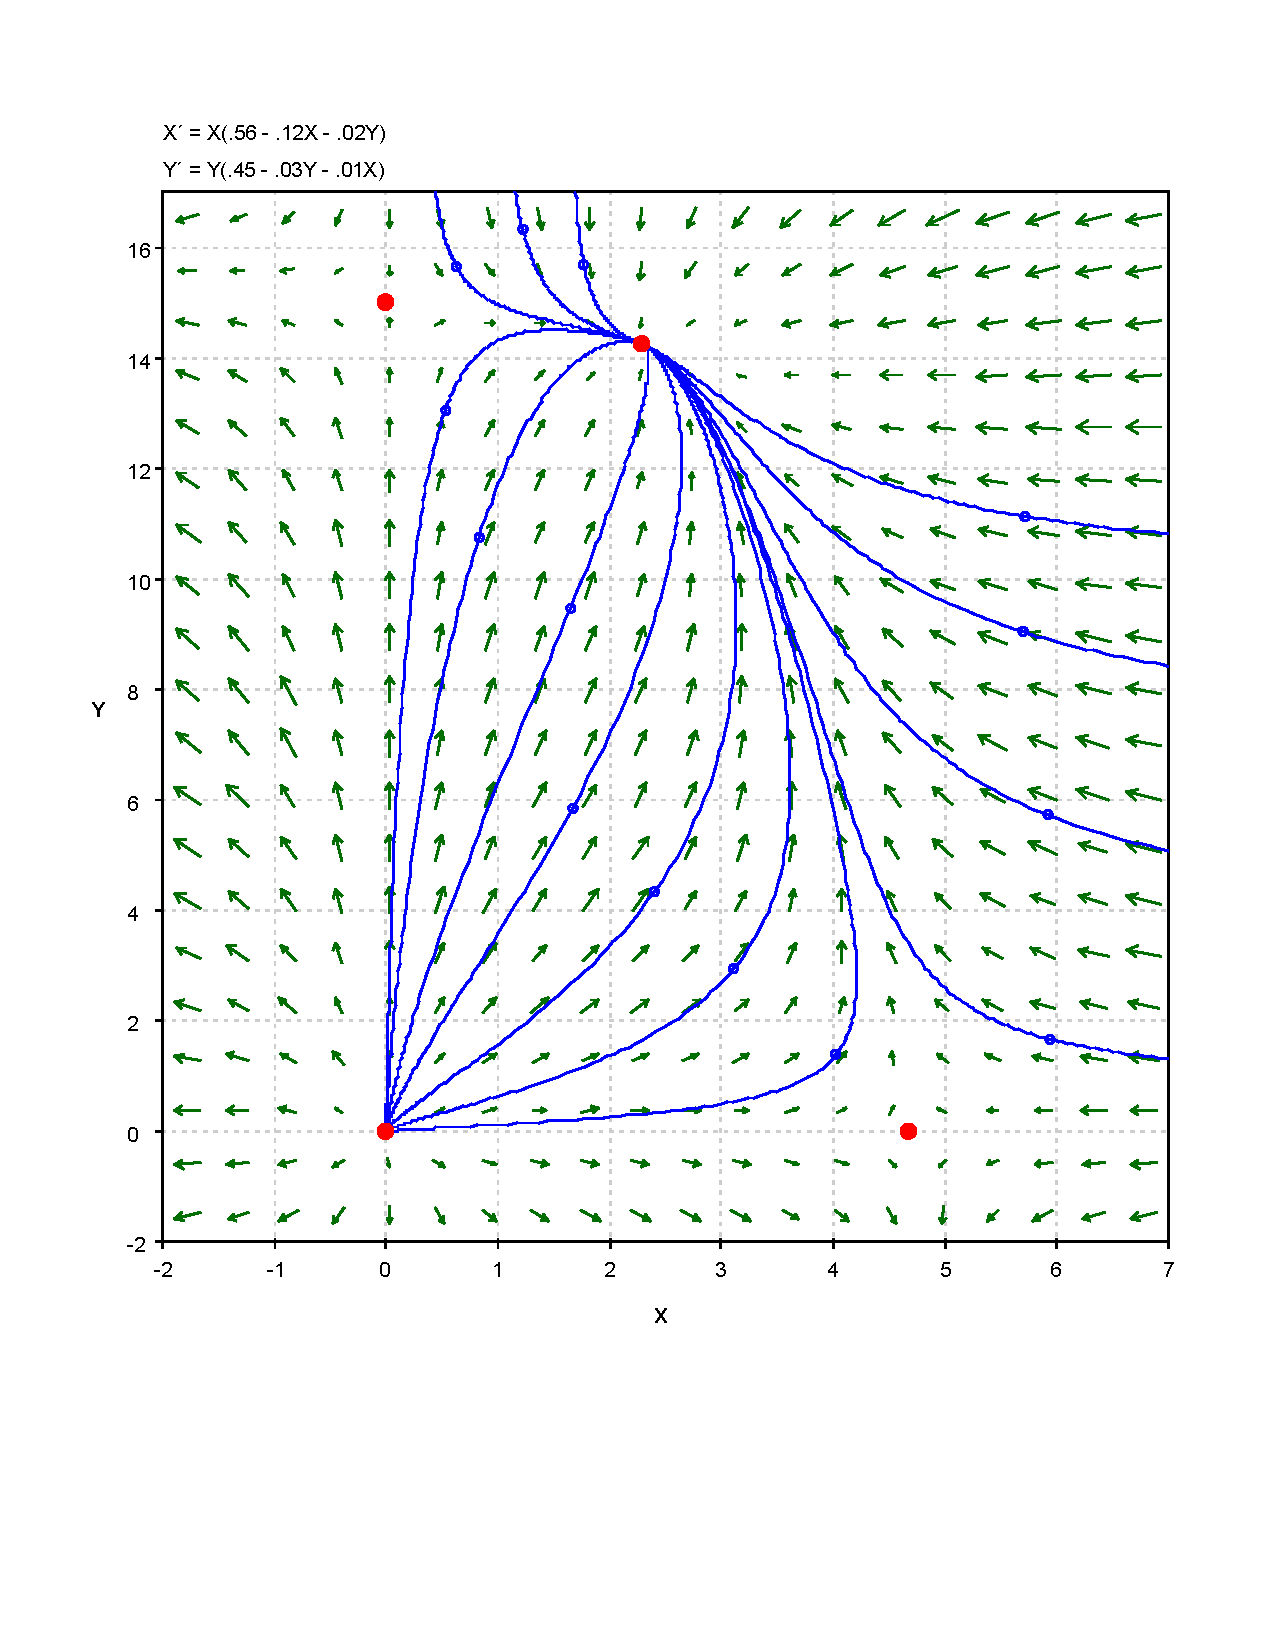
\includegraphics[width = 16cm]{Prob4.png}
			\end{figure}
			\skipline
			\skipline
			Notice when both species are extinct, they each grow to co-exist.  The start at (0,0) and go away from that point because it is a source.  When one species is extinct, the population tends near it then reverts to the co-existence point.  That is because they are saddle points. Lastly, when both species co-exist, all populations go towards this point because it is a sink.
		\end{enumerate}
	\end{problem}

\end{document}
